% \iffalse meta-comment
%
% Copyright (C) 2016 by Jose C. Pernias <jcpernias@gmail.com>
% -------------------------------------------------------
% 
% This file may be distributed and/or modified under the
% conditions of the LaTeX Project Public License, either version 1.3
% of this license or (at your option) any later version.
% The latest version of this license is in:
%
%    http://www.latex-project.org/lppl.txt
%
% and version 1.3 or later is part of all distributions of LaTeX 
% version 2005/12/01 or later.
%
% \fi
%
% \iffalse
%<*driver>
\ProvidesFile{jpmath.dtx}
%</driver>
%<package>\NeedsTeXFormat{LaTeX2e}[2005/12/01]
%<package>\ProvidesPackage{jpmath}
%<*package>
    [2016/03/01 v1.0 Macros for math]
%</package>
%
%<*driver>
\documentclass{ltxdoc}
\usepackage[parfill]{parskip}
\usepackage{fancyvrb}
\usepackage[T1]{fontenc}
\usepackage[full]{textcomp}
\usepackage[osf,sc]{mathpazo}
\renewcommand\sfdefault{lmss}
\renewcommand\ttdefault{lmtt}
%\usepackage[scaled]{luximono}
\usepackage{jpmath}[2016/03/01]
\usepackage{microtype}

\usepackage[skins,listings]{tcolorbox}
\newtcblisting{exampleB}[2][]{%
  colframe=red!50!yellow!50!black,
  colback=white,
  coltitle=red!50!yellow!3!white,
  bicolor,colbacklower=red!50!yellow!5!white,
  fonttitle=\sffamily\bfseries,
  sidebyside,text and listing,
  title=#2,#1}

\usepackage{url}
\usepackage{hyperref}
\usepackage{bookmark}
\EnableCrossrefs         
\CodelineIndex
\RecordChanges
\begin{document}
  \DocInput{jpmath.dtx}
  \PrintChanges
  \PrintIndex
\end{document}
%</driver>
% \fi
%
% \CheckSum{0}
%
% \CharacterTable
%  {Upper-case    \A\B\C\D\E\F\G\H\I\J\K\L\M\N\O\P\Q\R\S\T\U\V\W\X\Y\Z
%   Lower-case    \a\b\c\d\e\f\g\h\i\j\k\l\m\n\o\p\q\r\s\t\u\v\w\x\y\z
%   Digits        \0\1\2\3\4\5\6\7\8\9
%   Exclamation   \!     Double quote  \"     Hash (number) \#
%   Dollar        \$     Percent       \%     Ampersand     \&
%   Acute accent  \'     Left paren    \(     Right paren   \)
%   Asterisk      \*     Plus          \+     Comma         \,
%   Minus         \-     Point         \.     Solidus       \/
%   Colon         \:     Semicolon     \;     Less than     \<
%   Equals        \=     Greater than  \>     Question mark \?
%   Commercial at \@     Left bracket  \[     Backslash     \\
%   Right bracket \]     Circumflex    \^     Underscore    \_
%   Grave accent  \`     Left brace    \{     Vertical bar  \|
%   Right brace   \}     Tilde         \~}
%
%
% \changes{v1.0}{2016/03/01}{Initial version}
%
% \GetFileInfo{jpmath.dtx}
%
% \DoNotIndex{\newcommand,\newenvironment,\frac,\RequirePackage}
% \DoNotIndex{\def,\if,\else,\fi,\ifcat,\ifdim,\csname,\endcsname,\expandafter}
% \DoNotIndex{\advance,\begingroup,\endgroup,\let,\relax,\ht,\wd,\noexpand,\futurelet}
% \DoNotIndex{\DeclareDocumentCommand,\IfBooleanTF,\IfNoValueTF,\IfValueTF}
% \DoNotIndex{\mathtoolset,\DeclarePairedDelimiter}
% \DoNotIndex{\overline,\quad,\mathop,\mathrm,\lvert,\rvert,\mathaccent,\mathaccentV}
% \DoNotIndex{\mathsurround,\mathgroup}
% \DoNotIndex{\macc@depth}
% \DoNotIndex{\endmarker}
% \DoNotIndex{\text,\textit,\textnormal,\scriptspace}
% \DoNotIndex{\hbox,\setbox,\savebox,\dimen@,\dimexpr,\divide,\kern,\rel@kern}
% \DoNotIndex{\translate,\deftranslation}
% \DoNotIndex{\,,\!,\%}
% 
%
% \title{The \textsf{jpmath} package\thanks{This document
%   corresponds to \textsf{jpmath}~\fileversion, dated \filedate.}}
% \author{Jos\'e C. Pern\'{\i}as \\ \texttt{jcpernias@gmail.com}}
%
% \maketitle
%
% \section{Introduction}
%
% Put text here.
%
% \section{Usage}
%
% Put text here.
% 
% \DescribeMacro{\mname}
% This macro does nothing.\index{naming|usage} It is merely an
% example.  If this were a real macro, you would put a paragraph here
% describing what the macro is supposed to do, what its mandatory and
% optional arguments are, and so forth.
%
% \DescribeMacro{\widebar}
% A replacement for \cs{bar}:
% \begin{Verbatim}[frame=single,commandchars=\|\[\],gobble=2,fontfamily=tt]
% |cs[widebar]|marg[text]
% \end{Verbatim}
% For example \cs{widebar\{\cs{beta}\cs{omega}\}} produces:
% \begin{equation*}
%   \widebar{\beta \omega}
% \end{equation*}
% 
% \iffalse
%<*example>
% \fi

\begin{exampleB}[lefthand width=3.5cm]{}
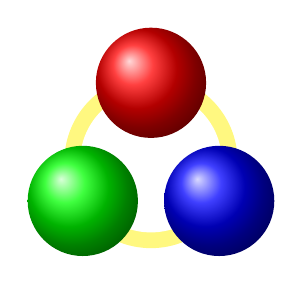
\begin{tikzpicture}
\path[fill=yellow!50!white] (0,0) circle (11mm);
\path[fill=white] (0,0) circle (9mm);
\foreach \w/\c in {90/red,210/green,330/blue}
{\path[shading=ball,ball color=\c] (\w:1cm) circle (7mm);}
\end{tikzpicture}
\end{exampleB}

% \iffalse
%</example>
% \fi
% \StopEventually{\PrintChanges\PrintIndex}
%
% \section{Implementation}
%

% 
% Load required packages:
%    \begin{macrocode}
\RequirePackage{latexsym}
\RequirePackage{amssymb}
\RequirePackage{mathtools}
\mathtoolsset{mathic}
\RequirePackage{xparse}
%    \end{macrocode}
%
% \begin{macro}{\qtext}
%   Enclose text between two \cs{quad}'s
%    \begin{macrocode}
\newcommand*{\qtext}[1]{\quad\text{#1}\quad}
%    \end{macrocode}
% \end{macro}
% 
% \begin{macro}{\mname}
%   Macro for defining function names.
%
%   While we're at it, please allow me to point out that when
%   "romanizing" multi-letter suffixes (like, say, "fin" for "final"),
%   it's advisable to go for \cs{textnormal} rather than \cs{mathrm},
%   because the latter just renders a bunch of Roman characters
%   side-by-side, without optimizing the spacing to make them look
%   like the abbreviation to a single word.
%
%   Therefore you use \cs{textnormal} for sin, but \cs{text} for if
%   and only if. The reason is that sin should be upright even in for
%   instance a theorem statement, whereas if and only if as a part of
%   a displayed equation should be italic in a theorem statement
%   (given you typeset theorems in italics)
%
%    \begin{macrocode}
\DeclareDocumentCommand \mname { s o m } { \mathop{}\!%
  \IfBooleanTF{#1}{ %
    \IfValueTF{#2} {%
%    \end{macrocode}
% Starred with subscript
%    \begin{macrocode}
      \textnormal{#3}_{\textnormal{#2}} }{%
%    \end{macrocode}
% Starred without subscript
%    \begin{macrocode}
      \textnormal{#3} } }{%
    \IfValueTF{#2} {%
%    \end{macrocode}
% Unstarred with subscript
%    \begin{macrocode}
      \textnormal{\textit{#3}}_{\textnormal{#2}} }{%
%    \end{macrocode}
% Unstarred without subscript
%    \begin{macrocode}
      \textnormal{\textit{#3}} } } }
%    \end{macrocode}
% \end{macro}


% \begin{macro}{\widebar}
% Replacement for bar: from a post by Hendrik Vogt:
% \url{http://tex.stackexchange.com/a/60253}
%    \begin{macrocode}
\let\save@mathaccent\mathaccent
\newcommand*\if@single[3]{%
  \setbox0\hbox{${\mathaccent"0362{#1}}^H$}%
  \setbox2\hbox{${\mathaccent"0362{\kern0pt#1}}^H$}%
  \ifdim\ht0=\ht2 #3\else #2\fi
  }
%    \end{macrocode}
% The bar will be moved to the right by a half of \cs{macc@kerna}, 
% which is computed by amsmath:
%    \begin{macrocode}
\newcommand*\rel@kern[1]{\kern#1\dimexpr\macc@kerna}
%    \end{macrocode}
% If there's a superscript following the bar, then no negative kern
% may follow the bar; an additional \{\} makes sure that the
% superscript is high enough in this case:
%    \begin{macrocode}
\newcommand*\widebar[1]{\@ifnextchar^{{\wide@bar{#1}{0}}}{\wide@bar{#1}{1}}}
%    \end{macrocode}
% Use a separate algorithm for single symbols:
%    \begin{macrocode}
\newcommand*\wide@bar[2]{\if@single{#1}{\wide@bar@{#1}{#2}{1}}{\wide@bar@{#1}{#2}{2}}}
\newcommand*\wide@bar@[3]{%
  \begingroup
  \def\mathaccent##1##2{%
%    \end{macrocode}
% Enable nesting of accents:
%    \begin{macrocode}
    \let\mathaccent\save@mathaccent
%    \end{macrocode}
% If there's more than a single symbol, use the first character instead (see below):
%    \begin{macrocode}
    \if#32 \let\macc@nucleus\first@char \fi
%    \end{macrocode}
% Determine the italic correction:
%    \begin{macrocode}
    \setbox\z@\hbox{$\macc@style{\macc@nucleus}_{}$}%
    \setbox\tw@\hbox{$\macc@style{\macc@nucleus}{}_{}$}%
    \dimen@\wd\tw@
    \advance\dimen@-\wd\z@
%    \end{macrocode}
% Now \cs{dimen@} is the italic correction of the symbol.
%    \begin{macrocode}
    \divide\dimen@ 3
    \@tempdima\wd\tw@
    \advance\@tempdima-\scriptspace
%    \end{macrocode}
% Now \cs{@tempdima} is the width of the symbol.
%    \begin{macrocode}
    \divide\@tempdima 10
    \advance\dimen@-\@tempdima
%    \end{macrocode}
% Now \cs{dimen@} = (italic correction / 3) - (Breite / 10)
%    \begin{macrocode}
    \ifdim\dimen@>\z@ \dimen@0pt\fi
%    \end{macrocode}
% The bar will be shortened in the case \cs{dimen@}<0 !
%    \begin{macrocode}
    \rel@kern{0.6}\kern-\dimen@
    \if#31
      \overline{\rel@kern{-0.6}\kern\dimen@\macc@nucleus\rel@kern{0.4}\kern\dimen@}%
      \advance\dimen@0.4\dimexpr\macc@kerna
%    \end{macrocode}
% Place the combined final kern (-\cs{dimen@}) if it is >0 or if a superscript follows:
%    \begin{macrocode}
      \let\final@kern#2%
      \ifdim\dimen@<\z@ \let\final@kern1\fi
      \if\final@kern1 \kern-\dimen@\fi
    \else
      \overline{\rel@kern{-0.6}\kern\dimen@#1}%
    \fi
  }%
  \macc@depth\@ne
  \let\math@bgroup\@empty \let\math@egroup\macc@set@skewchar
  \mathsurround\z@ \frozen@everymath{\mathgroup\macc@group\relax}%
  \macc@set@skewchar\relax
  \let\mathaccentV\macc@nested@a
%    \end{macrocode}
% The following initialises \cs{macc@kerna} and calls \cs{mathaccent}:
%    \begin{macrocode}
  \if#31
    \macc@nested@a\relax111{#1}%
  \else
%    \end{macrocode}
% If the argument consists of more than one symbol, and if the first token is
% a letter, use that letter for the computations:
%    \begin{macrocode}
    \def\gobble@till@marker##1\endmarker{}%
    \futurelet\first@char\gobble@till@marker#1\endmarker
    \ifcat\noexpand\first@char A\else
      \def\first@char{}%
    \fi
    \macc@nested@a\relax111{\first@char}%
  \fi
  \endgroup
}
%    \end{macrocode}
% \end{macro}
%
% \begin{macro}{\diff}
%   diff operator
%    \begin{macrocode}
\newcommand*{\diff}{\mathop{}\!\mathrm{d}}
%    \end{macrocode}
% \end{macro}
%
% \begin{macro}{\deriv}
%   Derivatives:
%    \begin{macrocode}
\DeclareDocumentCommand \deriv { o m g } {%
  \IfNoValueTF{#1} {%
%    \end{macrocode}
% No Power
%    \begin{macrocode}
    \IfNoValueTF{#3} {%
%    \end{macrocode}
% Without f(x)
%    \begin{macrocode}
      \frac{\diff}{\diff #2}\, }{%
%    \end{macrocode}
% With f(x)
%    \begin{macrocode}
      \frac{\diff #2}{\diff #3} } }{%
%    \end{macrocode}
% Power
%    \begin{macrocode}
    \IfNoValueTF{#3} {%
%    \end{macrocode}
% Without f(x)
%    \begin{macrocode}
      \frac{\diff^{#1}}{\diff #2^{#1}}\, }{%
%    \end{macrocode}
% With f(x)
%    \begin{macrocode}
      \frac{\diff^{#1} #2}{\diff #3^{#1}} } } }
%    \end{macrocode}
% \end{macro}
%
% \begin{macro}{\pderiv}
%   Partial dervatives:
%    \begin{macrocode}
\DeclareDocumentCommand \pderiv { o m g } {%
  \IfNoValueTF{#1} {%
%    \end{macrocode}
% No Power
%    \begin{macrocode}
    \IfNoValueTF{#3} {%
%    \end{macrocode}
% Without f(x)
%    \begin{macrocode}
      \frac{\partial}{\partial #2}\, }{%
%    \end{macrocode}
% With f(x)
%    \begin{macrocode}
      \frac{\partial #2}{\partial #3} } }{%
%    \end{macrocode}
% Power
%    \begin{macrocode}
    \IfNoValueTF{#3} {%
%    \end{macrocode}
% Without f(x)
%    \begin{macrocode}
      \frac{\partial^{#1}}{\partial #2^{#1}}\, }{%
%    \end{macrocode}
% With f(x)
%    \begin{macrocode}
      \frac{\partial^{#1} #2}{\partial #3^{#1}} } } }
%    \end{macrocode}
% \end{macro}
%
% \begin{macro}{\pxderiv}
%   Cross partial derivatives
%    \begin{macrocode}
\DeclareDocumentCommand \pxderiv { m m g } {%
  \IfNoValueTF{#3} {%
%    \end{macrocode}
% Without f(x)
%    \begin{macrocode}
    \frac{\partial^2}{\partial #1\, \partial #2}\, }{%
%    \end{macrocode}
% With f(x)
%    \begin{macrocode}
    \frac{\partial^2 #1}{\partial #2\, \partial #3} } }
%    \end{macrocode}
% \end{macro}

% \begin{macro}{\incr}
%   Increment operator
%    \begin{macrocode}
\newcommand*{\incr}{\mathop{}\!\Delta}
%    \end{macrocode}
% \end{macro}
%
% \begin{macro}{\incrpct}
%   Percent increment operator
%    \begin{macrocode}
\newcommand*{\incrpct}{\mathop{}\!\Delta\%}
%    \end{macrocode}
% \end{macro}
%
% \begin{macro}{\iratio}
%   Increment ratio
%    \begin{macrocode}
\newcommand*{\iratio}[2]{\frac{\incr #1}{\incr #2}}
%    \end{macrocode}
% \end{macro}
%
% \begin{macro}{\ipctratio}
%   Percent increment ratio
%    \begin{macrocode}
\newcommand*{\ipctratio}[2]{\frac{\incrpct #1}{\incrpct #2}}
%    \end{macrocode}
% \end{macro}
% 
% \begin{macro}{\abs}
%   Absolute value
%    \begin{macrocode}
\DeclarePairedDelimiter\jpmath@abs{\lvert}{\rvert}
\newcommand*{\abs}[1]{\jpmath@abs*{#1}}
%    \end{macrocode}
% \end{macro}
%
% \begin{macro}{\eval}
%   Evaluation:
%    \begin{macrocode}
\DeclarePairedDelimiter\jpmath@eval{.}{\rvert}
\newcommand*{\eval}[2]{\jpmath@eval*{#1}_{#2}}
%    \end{macrocode}
% \end{macro}
%
% \Finale
% \endinput


% Local Variables:
% mode: doctex
% TeX-master: nil
% End:
